\documentclass{standalone}
\usepackage{tikz}
\usetikzlibrary{patterns, positioning}
\usepackage[sfdefault]{ClearSans} %% option 'sfdefault' activates Clear Sans as the default text font
\usepackage[T1]{fontenc}

\begin{document}
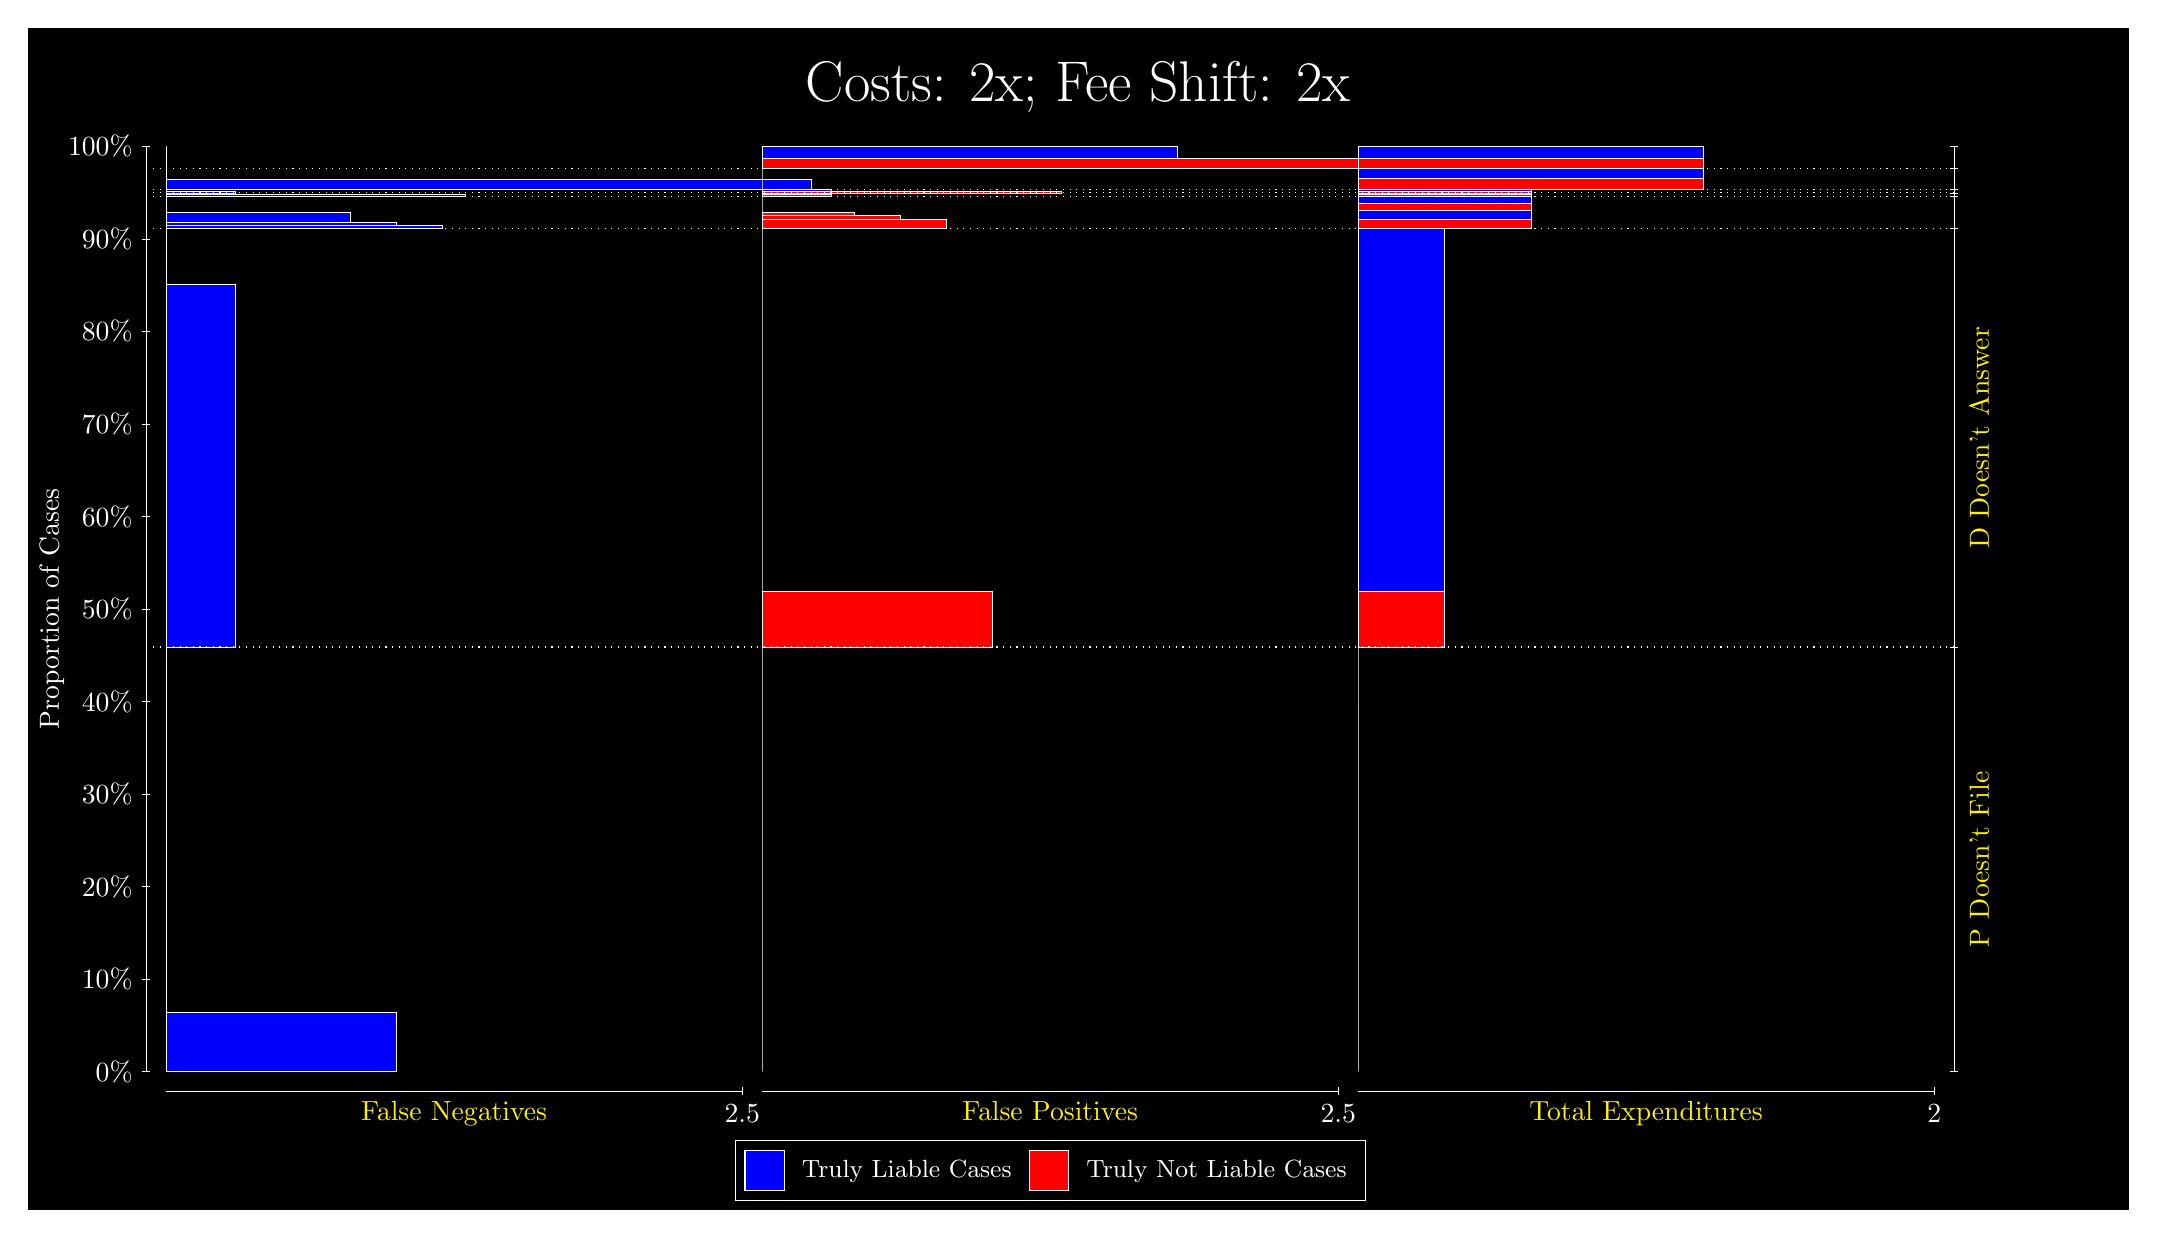
\begin{tikzpicture}
\draw[fill=black] (0,0) rectangle (26.667,15);
\draw[text=white] (0,13.5) rectangle (26.667,15) node[midway] {\huge Costs: 2x; Fee Shift: 2x};
\draw[white, very thin] (1.5,1.75) -- (1.5,13.5);
\node[rotate=90, text=white, anchor=center] at (0.3, 7.625) {Proportion of Cases};
\draw[white, very thin] (1.45,1.75) -- (1.55,1.75);
\node[text=white, anchor=east] at (1.45, 1.75) {0\%};
\draw[white, very thin] (1.45,2.925) -- (1.55,2.925);
\node[text=white, anchor=east] at (1.45, 2.925) {10\%};
\draw[white, very thin] (1.45,4.1) -- (1.55,4.1);
\node[text=white, anchor=east] at (1.45, 4.1) {20\%};
\draw[white, very thin] (1.45,5.275) -- (1.55,5.275);
\node[text=white, anchor=east] at (1.45, 5.275) {30\%};
\draw[white, very thin] (1.45,6.45) -- (1.55,6.45);
\node[text=white, anchor=east] at (1.45, 6.45) {40\%};
\draw[white, very thin] (1.45,7.625) -- (1.55,7.625);
\node[text=white, anchor=east] at (1.45, 7.625) {50\%};
\draw[white, very thin] (1.45,8.8) -- (1.55,8.8);
\node[text=white, anchor=east] at (1.45, 8.8) {60\%};
\draw[white, very thin] (1.45,9.975) -- (1.55,9.975);
\node[text=white, anchor=east] at (1.45, 9.975) {70\%};
\draw[white, very thin] (1.45,11.15) -- (1.55,11.15);
\node[text=white, anchor=east] at (1.45, 11.15) {80\%};
\draw[white, very thin] (1.45,12.325) -- (1.55,12.325);
\node[text=white, anchor=east] at (1.45, 12.325) {90\%};
\draw[white, very thin] (1.45,13.5) -- (1.55,13.5);
\node[text=white, anchor=east] at (1.45, 13.5) {100\%};

\draw[white, very thin] (24.457,1.75) -- (24.457,13.5);
\draw[white, very thin] (24.407,1.75) -- (24.507,1.75);
\node[anchor=west] at (24.407, 1.75) {};
\draw[white, very thin] (24.407,7.1418) -- (24.507,7.1418);
\node[anchor=west] at (24.407, 7.1418) {};
\draw[white, very thin] (24.407,12.456) -- (24.507,12.456);
\node[anchor=west] at (24.407, 12.456) {};
\draw[white, very thin] (24.407,12.865) -- (24.507,12.865);
\node[anchor=west] at (24.407, 12.865) {};
\draw[white, very thin] (24.407,12.91) -- (24.507,12.91);
\node[anchor=west] at (24.407, 12.91) {};
\draw[white, very thin] (24.407,12.952) -- (24.507,12.952);
\node[anchor=west] at (24.407, 12.952) {};
\draw[white, very thin] (24.407,13.223) -- (24.507,13.223);
\node[anchor=west] at (24.407, 13.223) {};
\draw[white, very thin] (24.407,13.5) -- (24.507,13.5);
\node[anchor=west] at (24.407, 13.5) {};

\draw[white, very thin, fill=blue] (1.75,1.75) rectangle (4.6775,2.5017);
\draw[white, very thin, fill=red] (1.75,2.5017) rectangle (1.75,7.1418);
\draw[white, very thin, fill=blue] (1.75,7.1418) rectangle (2.6283,11.743);
\draw[white, very thin, fill=red] (1.75,11.743) rectangle (1.75,12.456);
\draw[white, very thin, fill=blue] (1.75,12.456) rectangle (5.2631,12.491);
\draw[white, very thin, fill=blue] (1.75,12.491) rectangle (4.6775,12.539);
\draw[white, very thin, fill=blue] (1.75,12.539) rectangle (4.092,12.659);
\draw[white, very thin, fill=red] (1.75,12.659) rectangle (1.75,12.865);
\draw[white, very thin, fill=blue] (1.75,12.865) rectangle (5.5558,12.886);
\draw[white, very thin, fill=red] (1.75,12.886) rectangle (1.75,12.91);
\draw[white, very thin, fill=blue] (1.75,12.91) rectangle (2.6283,12.932);
\draw[white, very thin, fill=red] (1.75,12.932) rectangle (1.75,12.952);
\draw[white, very thin, fill=blue] (1.75,12.952) rectangle (9.9471,13.078);
\draw[white, very thin, fill=red] (1.75,13.078) rectangle (1.75,13.223);
\draw[white, very thin, fill=red] (1.75,13.223) rectangle (1.75,13.351);
\draw[white, very thin, fill=blue] (1.75,13.351) rectangle (1.75,13.5);
\draw[white, very thin, fill=red] (9.3189,1.75) rectangle (9.3189,6.39);
\draw[white, very thin, fill=blue] (9.3189,6.39) rectangle (9.3189,7.1418);
\draw[white, very thin, fill=red] (9.3189,7.1418) rectangle (12.246,7.8546);
\draw[white, very thin, fill=blue] (9.3189,7.8546) rectangle (9.3189,12.456);
\draw[white, very thin, fill=red] (9.3189,12.456) rectangle (11.661,12.575);
\draw[white, very thin, fill=red] (9.3189,12.575) rectangle (11.075,12.624);
\draw[white, very thin, fill=red] (9.3189,12.624) rectangle (10.49,12.662);
\draw[white, very thin, fill=blue] (9.3189,12.662) rectangle (9.3189,12.865);
\draw[white, very thin, fill=red] (9.3189,12.865) rectangle (10.197,12.889);
\draw[white, very thin, fill=blue] (9.3189,12.889) rectangle (9.3189,12.91);
\draw[white, very thin, fill=red] (9.3189,12.91) rectangle (13.125,12.929);
\draw[white, very thin, fill=blue] (9.3189,12.929) rectangle (10.197,12.952);
\draw[white, very thin, fill=red] (9.3189,12.952) rectangle (9.3189,13.097);
\draw[white, very thin, fill=blue] (9.3189,13.097) rectangle (9.3189,13.223);
\draw[white, very thin, fill=red] (9.3189,13.223) rectangle (17.516,13.351);
\draw[white, very thin, fill=blue] (9.3189,13.351) rectangle (14.588,13.5);
\draw[white, very thin, fill=red] (16.888,1.75) rectangle (16.888,6.39);
\draw[white, very thin, fill=blue] (16.888,6.39) rectangle (16.888,7.1418);
\draw[white, very thin, fill=red] (16.888,7.1418) rectangle (17.986,7.8546);
\draw[white, very thin, fill=blue] (16.888,7.8546) rectangle (17.986,12.456);
\draw[white, very thin, fill=red] (16.888,12.456) rectangle (19.083,12.575);
\draw[white, very thin, fill=blue] (16.888,12.575) rectangle (19.083,12.694);
\draw[white, very thin, fill=red] (16.888,12.694) rectangle (19.083,12.781);
\draw[white, very thin, fill=blue] (16.888,12.781) rectangle (19.083,12.865);
\draw[white, very thin, fill=red] (16.888,12.865) rectangle (19.083,12.889);
\draw[white, very thin, fill=blue] (16.888,12.889) rectangle (19.083,12.91);
\draw[white, very thin, fill=red] (16.888,12.91) rectangle (19.083,12.929);
\draw[white, very thin, fill=blue] (16.888,12.929) rectangle (19.083,12.952);
\draw[white, very thin, fill=red] (16.888,12.952) rectangle (21.279,13.097);
\draw[white, very thin, fill=blue] (16.888,13.097) rectangle (21.279,13.223);
\draw[white, very thin, fill=red] (16.888,13.223) rectangle (21.279,13.351);
\draw[white, very thin, fill=blue] (16.888,13.351) rectangle (21.279,13.5);
\draw[white, dotted] (1.5,7.1418) -- (24.457,7.1418);
\draw[white, dotted] (1.5,12.456) -- (24.457,12.456);
\draw[white, dotted] (1.5,12.865) -- (24.457,12.865);
\draw[white, dotted] (1.5,12.91) -- (24.457,12.91);
\draw[white, dotted] (1.5,12.952) -- (24.457,12.952);
\draw[white, dotted] (1.5,13.223) -- (24.457,13.223);
\draw[white, very thin] (1.75,1.5) -- (9.0689,1.5);
\node[text=yellow, anchor=north] at (5.4094, 1.5) {False Negatives};
\draw[white, very thin] (9.0689,1.45) -- (9.0689,1.55);
\node[text=white, anchor=north] at (9.0689, 1.45) {2.5};

\draw[white, very thin] (9.3189,1.5) -- (16.638,1.5);
\node[text=yellow, anchor=north] at (12.978, 1.5) {False Positives};
\draw[white, very thin] (16.638,1.45) -- (16.638,1.55);
\node[text=white, anchor=north] at (16.638, 1.45) {2.5};

\draw[white, very thin] (16.888,1.5) -- (24.207,1.5);
\node[text=yellow, anchor=north] at (20.547, 1.5) {Total Expenditures};
\draw[white, very thin] (24.207,1.45) -- (24.207,1.55);
\node[text=white, anchor=north] at (24.207, 1.45) {2};

\node[text=yellow, centered, rotate=90] at (24.777, 4.4459) {P Doesn't File};
\node[text=yellow, centered, rotate=90] at (24.777, 9.7987) {D Doesn't Answer};






\draw (12.978300999999998,1.5) node[draw=none] (baseCoordinate) {};
\begin{scope}[align=center]
        \matrix[scale=0.5, draw=white, below=0.5cm of baseCoordinate, nodes={draw}, column sep=0.1cm]{
            \node[rectangle, draw, minimum width=0.5cm, minimum height=0.5cm, fill=blue] {}; &
            \node[draw=none, font=\small, text=white] (B) {Truly Liable Cases}; &
            \node[rectangle, draw, minimum width=0.5cm, minimum height=0.5cm, fill=red] {}; &
            \node[draw=none, font=\small, text=white] (B) {Truly Not Liable Cases}; \\
            };
\end{scope}

\end{tikzpicture}
\end{document}